\documentclass[12pt, a4paper, oneside]{ctexart}
\usepackage{amsmath, amsthm, amssymb, bm, color, graphicx, geometry, hyperref, mathrsfs,extarrows, braket, booktabs, array}
\setmainfont{Times New Roman}  % 设置英文字体
\setsansfont{Calibri}
\setmonofont{Consolas}

\linespread{1.4}
%\geometry{left=2.54cm,right=2.54cm,top=3.18cm,bottom=3.18cm}
\geometry{left=1.84cm,right=1.84cm,top=2.18cm,bottom=2.18cm}
\newenvironment{problem}{\par\noindent\textbf{题目. }}{\bigskip\par}
\newenvironment{solution}{\par\noindent\textbf{解答. }}{\bigskip\par}
\newenvironment{note}{\par\noindent\textbf{注记. }}{\bigskip\par}

\everymath{\displaystyle} % 默认全部行间公式
\DeclareMathOperator*\uplim{\overline{lim}} % 定义上极限 \uplim_{}
\DeclareMathOperator*\lowlim{\underline{lim}} % 定义下极限 \lowlim_{}
\let\leq=\leqslant % 将全部leq变为leqslant
\let\geq=\geqslant % geq同理

% 一些宏定义
\def\bd{\boldsymbol}    % 加粗(向量) boldsymbol
\def\disp{\displaystyle}% 使用行间公式 displaystyle(默认)
\def\tsty{\textstyle}   % 使用行内公式 textstyle
\def\sign{\text{sign}}  % sign function
\def\wtd{\widetilde}    % 宽波浪线 widetilde
\def\R{\mathbb{R}}      % Real number
\def\C{\mathbb{C}}      % Complex number
\def\d{\mathrm{d}}      % differential operator
\def\e{\mathrm{e}}      % Euler's number
\def\i{\mathrm{i}}      % imaginary number
\def\L{\bd{L}}          % Lebesgue可测集
\def\wdh{\widehat}      % 宽帽子 widehat
\def\ol{\overline}      % 上横线 overline
\def\ul{\underline}     % 下横线 underline
\def\add{\vspace{0.5ex}}  % 增加行间距
\def\del{\vspace{-2.5ex}}  % 减少行间距

% 基本信息
\newcommand{\RQ}{\today} % 日期
\newcommand{\km}{实变函数} % 科目
\newcommand{\bj}{强基数学002} % 班级
\newcommand{\xm}{吴天阳} % 姓名
\newcommand{\xh}{2204210460} % 学号
\newcommand{\XH}{59} % 序号

\begin{document}

%\pagestyle{empty}
\pagestyle{plain}
\vspace*{-15ex}
\centerline{\begin{tabular}{*6{c}}
    \parbox[t]{0.25\linewidth}{\begin{center}\textbf{日期}\\ \large \textcolor{blue}{\RQ}\end{center}} 
    & \parbox[t]{0.15\linewidth}{\begin{center}\textbf{科目}\\ \large \textcolor{blue}{\km}\end{center}}
    & \parbox[t]{0.2\linewidth}{\begin{center}\textbf{班级}\\ \large \textcolor{blue}{\bj}\end{center}}
    & \parbox[t]{0.1\linewidth}{\begin{center}\textbf{姓名}\\ \large \textcolor{blue}{\xm}\end{center}}
    & \parbox[t]{0.15\linewidth}{\begin{center}\textbf{学号}\\ \large \textcolor{blue}{\xh}\end{center}}
    & \parbox[t]{0.1\linewidth}{\begin{center}\textbf{序号}\\ \large \textcolor{blue}{\XH}\end{center}} \\ \hline
\end{tabular}}
\vspace*{4ex}

% 正文部分
\del
\paragraph{习题 2.4}
\paragraph{1.}证明$[0,1]$上Cantor集的Lebesgue测度是零.
\begin{proof}
    令$C$为$[0,1]$上的Cantor集, 则$m^*([0,1] - C) = \frac{1}{3}+\frac{2^1}{3^2} + \frac{2^2}{3^3}+\cdots = \frac{\frac{1}{3}}{1-\frac{2}{3}} = 1$, 所以$m^*(C) = m^*([0,1]) - m^*([0, 1] - C) = 1-1 = 0$.
\end{proof}
\paragraph{2.}设$g(x)$是$(-\infty, \infty)$上单调增加右连续函数, $\bd{L}^g$是关于$g$的Lebesgue-Stieltjes可测集类, $g$是$\bd{L}^g$上Lebesgue-Stieltjes测度. 证明

(i) $g(\{a\}) = g(a) - g(a-0);\ g((a,b)) = g(b-0) - g(a);\ g([a, b]) = g(b) - g(a-0);\ g([a, b)) = g(b-0) - g(a-0);$ 

当开集$O = \bigcup_\nu(a_\nu, b_\nu)\ (\{(a_\nu, b_\nu)\}$是$O$的构成区间全体)时, $g(O) = \sum_{\nu}(g(b_\nu - 0) - g(a_\nu))$.

(ii) 引理2. 定理2.4.5-2.4.9对于$\bd{L}^g,\ g$也成立.
\begin{proof}
    \begin{align*}
        \text{(i)}\ g(\{a\}) =&\ g\left(\bigcap_{n=0}^{\infty}\left(a-\frac{1}{n}, a+\frac{1}{n}\right)\right) = \lim_{n\to \infty}g(a+\frac{1}{n})-g(a-\frac{1}{n}) = g(a) - g(a-0), \\
        g([a, b]) =&\ g\left(\bigcap_{n=1}^\infty(a-\frac{1}{n},b+\frac{1}{n})\right) = \lim_{n\to \infty}g(b+\frac{1}{n})-g(a-\frac{1}{n}) = g(b)-g(a-0),\\
        g((a, b)) =&\ g([a, b]) - g(\{a\}) - g(\{b\}) = g(b-0) - g(a),\\
        g([a, b)) =&\ g([a, b]) - g(\{b\}) = g(b-0) - g(a-0), \\
        g(O) =&\ g\left(\bigcup_{\nu}(a_\nu, b_\nu)\right) = \sum_\nu g(a_\nu, b_\nu) = \sum_\nu (g(b_\nu - 0) - g(a_\nu)).
    \end{align*}

    (ii) 证明与$\bd{L},\ m$情况完全一致, 只需将$m$换成$g$, $m^*$换成$g^*$.
\end{proof}
\paragraph{4.}设$g(x)$是$(-\infty, \infty)$上单调增加右连续函数.证明$g(x)$能够产生出Lebesgue可测集类$\bd{L}$上的测度$g$, 并且存在常数$\alpha$, 对一切$E\in\bd{L},\ g(E) = \alpha m(E)$成立的充要条件是$g(x) = \alpha x+c$, 这里$c$是常数.
\begin{proof}
    "$\Rightarrow$": 由于$g,\ m$均满足定理2.4.5, 存在开集$G$使得, $g(G) = g(E),\ m(G) = m(E)$, 设$(a_i, b_i)\ (i\in I)$为$G$的构成区间全体, 则
    \begin{align*}
        g(E) = g(G) = \sum_{i\in I}g((a_i, b_i)) = \sum_{i\in I}(g(b_i-0) - g(a_i)) = \alpha m(E) = \alpha \sum_{i\in I}(b_i-a_i)
    \end{align*}
    由于$a_i,\ b_i$的任意性, 可知$g(x)$在$\R$上是连续的, 不妨将$a_i$视为自变量$x$, 则$g'(x) = \alpha$, 于是$g(x) = \alpha x + c$.

    "$\Leftarrow$": 类似必要性证明, 任意的$E\in \bd{L}^g$, 取开集使得$g(G) = g(E)$, 则
    \begin{equation*}
        g(E) = g(G) = \sum_{i\in I}g((a_i, b_i)) = \sum_{i\in I}\alpha(b_i-a_i) = \alpha \sum_{i\in I}(b_i-a_i) = \alpha m(G) = \alpha m(E)
    \end{equation*}
    所以$m(G) = m(E)$, 则$E\in \bd{L}$, 所以$\bd{L}^g\subset \bd{L}$, 同理可证, $\bd{L}\subset \bd{L}^g$, 所以$\bd{L} = \bd{L}^g$, 且$g(E) = \alpha m(E)$.
\end{proof}
\paragraph{5.}\textbf{定义2.4.4}设$E$是直线上Lebesgue可测集, $x_0\in E$. 又设$(a, b)$是包含$x_0$的任一开区间. 如果下列极限存在
\begin{equation*}
    d = \lim_{(a, b)\to x_0}\frac{m((a, b)\cap E)}{b-a},
\end{equation*}
称$d$是$E$在点$x_0$的\textbf{密度}. 显然$0\leqslant d\leqslant 1$. 如果$d=1$, 称$x_0$是$E$的\textbf{全密点}.

(i) 点$a$是否是$E=[a, b]$的有密度的点.

(ii) 作一个集$E$, 使它在给定点$x_0$具有密度, 并且密度等于实现给定的值$c\ (0 < c < 1)$.\add
\begin{solution}
    (i) 不是, 因为$\lim_{n\to\infty}\frac{m((a-\frac{1}{n}, a+\frac{1}{n})\cap[a,b])}{\frac{2}{n}} = \lim_{n\to\infty}\frac{n}{2}\cdot m([a, a+\frac{1}{n})) = \frac{1}{2}$, 但\\$\lim_{n\to\infty}\frac{m((a-\frac{1}{n}, a+\frac{2}{n})\cap[a,b])}{\frac{3}{n}} = \lim_{n\to\infty}\frac{n}{3}\cdot m([a, a+\frac{2}{n})) = \frac{2}{3}\neq \frac{1}{2}$, 所以$a$不是$E$的有密度的点.

    (ii) 不妨令$x_0 = 0$, 仿照Cantor集构造方法, 在$(0, 1)$中取$\frac{1}{2}$为中点, 长度为$c_1$的区间, 在余下两个区间中取长度$c_1^2$的区间, 等等. 将这一列开区间记为$E_1$, 则$m(E_1) = c_1+2c_1^2+4c_1^3+\cdots=\frac{c_1}{1-2c_1}$, 对于任何$c\ (0 < c <1)$, 取$c_1$使得$\frac{c_1}{1-2c_1} = c$. 则$m(E_1) = c$. 类似的, 对Cantor集的余集$C^c$的每一个小区间$\Delta_i$, 作以上划分为$A_{\Delta_i}$, 可得$m(A_{\Delta_i}) = c\cdot m(\Delta_i)$, 将$(-1,0)$上对称的作出集合$B_{\Delta_j}$, 再令$E = \left(\bigcup_{i}A_{\Delta_i}\right)\cup\left(\bigcup_{j}B_{\Delta_j}\right)$, 则$E$满足题目要求.
\end{solution}\del
\paragraph{9.}举例说明引理$2$中的开集$O$不能换为闭集.
\begin{proof}
    令$E=\mathbb{Q}$, 取闭集$F$为全体有理点, 则$F^c$为只包含无理点的开集. 下证$F^c=\varnothing$.
    
    假设$F^c\neq \varnothing$, 则$\forall a\in F^c$, 满足$\exists \delta > 0$使得$(a-\delta, a + \delta)\subset F^c$. 由实数的稠密性可知, $\exists q$为有理数, 使得$q \in (a-\delta, a+\delta) \subset F^c$, 这与$F^c$中只有无理点矛盾, 所以$F^c = \varnothing$. 于是$F = \R$与$m^*(E) = 0$矛盾.
\end{proof}
\def\O{\bd{O}}
\def\F{\bd{F}}
\paragraph{11.}令$\O$为直线上开集全体, $\F$是直线上有界闭集全体. 作$\O\cup \F$上的集函数$\mu$如下: 当$\{(a_\nu, b_\nu)\}$是互不相交的开区间时,
\begin{equation*}
    \mu\left(\bigcup_{\nu}(a_\nu, b_\nu)\right) = \sum_{\nu}(b_\nu - a_\nu).
\end{equation*}
当$F\in\F$时, 如果$F\subset (a, b)$, 那么规定$\mu(F)  = b-a-\mu((a,b)-F)$. 对一切直线上的有界集$E$, 定义
\begin{equation*}
    \mu^*(E) = \inf\{\mu(O):E\subset O, O\in \O\},\ \mu_*(E) = \sup\{\mu(F):F\subset E, F\in\F\}.
\end{equation*}
当$\mu^*(E) = \mu_*(E)$时, 称$E$是可测集. 令$\L'$是可测集全体. 证明$\L'$是$\L$中有界集全体, 而且在$\L'$上$\mu^*=\mu_* = m^*$.
\begin{proof}
    规定: 下面证明中所涉及到的$a,b$均为有限数.
    
    设$\L^*$为$\L$中有界集全体, 即$\L^* = \{E\in \L:E\subset(a, b)\}$, 则命题等价于证明$\L^*=\L'$. 由于$\mu$在开集上的定义与$m$的定义相同, 所以根据\textbf{引理2}可知, $\mu^* = m^*$. 且对于任意的有界闭集$F$, 不妨令$F\subset (a, b)$, 则$\mu(F) = b-a-\mu((b-a)-F) = b-a-m((b-a)-F) = m(F)$.

    $\forall E\in \L^*$, 则$E$为$\L$-可测有限集, 不妨令$E\subset (a, b)$, $E_1 = (a, b)- E$, 则
    \begin{align*}
        \mu_*(E) =&\ \sup\{\mu(F):F\subset E,F\subset \F\} = \sup\{m(F):F\subset E, F\subset \F\}\\
        =&\ b-a-\inf\{m(O):E_1\subset O,O\subset \O\} = b-a-m^*(E_1) = m^*(E) = \mu^*(E).
    \end{align*}
    则$\mu_*(E) = \mu^*(E)$, 所以$E\in \L'$, 有$\L^*\subset \L'$.

    $\forall E\in \L'$, 则$\mu_*(E) = \mu^*(E)$, 由定义可知, $\forall \varepsilon > 0$, 存在开集$O$和闭集$F$使得, $F\subset E\subset O$ 且 
    \begin{equation*}
     \mu(O)-\varepsilon < \mu(E) < \mu(F) + \varepsilon   
    \end{equation*}
    则$\mu(O) - \mu(F) < 2\varepsilon$. 由于$O$和$F$均为Borel集, 于是$m(O) - m(F) < 2\varepsilon$, 则存在两个集列$\{O_n\}, \{F_n\}$, 满足$m(O_n) - m(F_n) < \frac{1}{n},\ (n=1,2,\cdots)$. 

    由于$\bigcup_{n=1}^\infty F_n\subset E\subset \bigcap_{n=1}^\infty O_n$, 则$\bigcap_{n=1}^\infty O_n - E\subset O_n - F_n$, 于是由测度的单调性可知
    \begin{equation*}
        m\left(\bigcap_{n=1}^\infty O_n - E\right)\leq m(O_n-F_n)\xlongequal{m\text{具有可加性}}m(O_n) - m(F_n) < \frac{1}{n}\to 0\quad (n\to \infty)
    \end{equation*}
    所以$\left(\bigcap_{n=1}^\infty O_n - E\right)$为Lebesgue零集.

    由于$E = \left(\bigcap_{n=1}^\infty O_n\right) - \left(\bigcap_{n=1}^\infty O_n - E\right)$, 所以$E$可以表示为Borel集和Lebesgue零集的差,\add 根据\textbf{定理2.4.9}可知,\add $E\in \L^*$, 有$\L'\subset \L^*$. 综上, $\L^* = \L'$.
\end{proof}
\paragraph{16.}设$m$是平面上的Lebesgue测度, $u_{\theta}$是平面上的一个映照(旋转):$(x, y)\mapsto (x', y')$,
\begin{equation*}
    x' = x\cos \theta+y\sin\theta,\ y'=-x\sin\theta+y\cos\theta.
\end{equation*}

证明: 对平面上任何Lebesgue可测集$E$, $u_{\theta}E$也Lebesgue可测集, 而且$m(u_{\theta}E) = m(E)$.
\begin{proof}
    由于$u_{\theta}$是双射, 则$E\in\L$, 任何的$F\subset \R^2$, 都有
    \begin{equation*}
        m^*(F) = m^*(F\cap E)+m^*(F-E)\Rightarrow 
        m^*(u_{\theta}F) = m^*(u_{\theta}F\cap u_{\theta}E)+m^*(u_{\theta}F-u_{\theta}E),
    \end{equation*}
    又由于$u_{\theta}F$是任意集, 所以$u_{\theta}E\in\L$.
    
    由Lebesgue积分可知
    \begin{equation*}
        m^*(u_{\theta}E) = \int_{u_{\theta}E}\,\d x\d y\xlongequal{u_{\theta}}\int_{E}|\det u_{\theta}|\,\d x\d y = \int_{E}\,\d x\d y = m^*(E)
    \end{equation*}
\end{proof}

% 下面给一些功能的写法
\iffalse
% 图片模板
\centerline{
    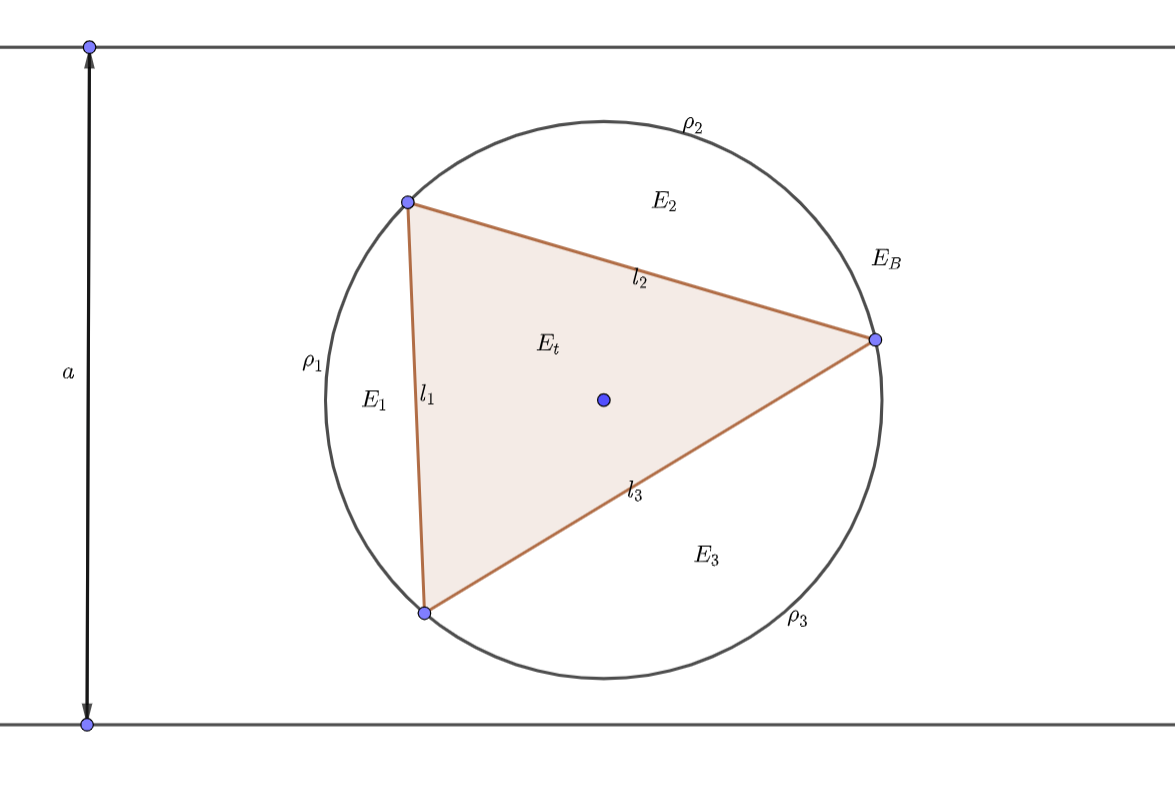
\includegraphics[width=0.8\textwidth]{figure.png}
}
% 表格模板
\renewcommand\arraystretch{0.8} % 设置表格高度为原来的0.8倍
\begin{table}[!htbp] % table标准
    \centering % 表格居中
    \begin{tabular}{p{1cm}<{\centering}p{1cm}<{\centering}p{3cm}<{\centering}p{5cm}<{\centering}} % 设置表格宽度
    %\begin{tabular}{cccc}
        \toprule
        $x_i$ & $f[x_1]$ & $f[x_i,x_{i+1}]$ & $f[x_i,x_{i+1},x_{i+2}]$ \\
        \midrule
        $x_0$ & $f(x_0)$ &                  &                          \\
        $x_0$ & $f(x_0)$ & $f'(x_0)$        &                          \\
        $x_0$ & $f(x_1)$ & $\frac{f(x_1)-f(x_0)}{x_1-x_0}$ & $\frac{f(x_1)-f(x_0)}{(x_1-x_0)^2}-\frac{f'(x_0)}{x_1-x_0}$\\
        \bottomrule
    \end{tabular}
\end{table}

\def\Log{\text{Log}} % 一个简单的宏定义
$\Log$ % 调用方法
\fi

\end{document}